\section{Формула Эйлера. Следствие}

Теорема \ref{theorem:chasles} доказана для любого \textit{конечного}
перемещения. Для частного случая \textit{бесконечно малого} перемещения дадим
векторную формулу. Для этого обозначим перемещение полюса $O'$ через
$\vec{p}_0$, а перемещение точки $M$ через $\vec{p}$; тогда
\begin{equation}
  \label{eq:flat_figure_movement_temp}
  \vec{p} = \vec{p}_0 + \vv{M' M_1}.
\end{equation}

Здесь $\vv{M' M_1}$ представляет собой перемещение точки $M$ при повороте фигуры
вокруг полюса. Обозначая угол поворота через $\theta$, будем иметь из
треугольника $O_1 M_1 M'$
\begin{equation*}
  M' M_1 = O_1 M' \cdot 2 \sin \frac{\theta}{2}.
\end{equation*}

Принимая поворот бесконечно малым, можно заменить синус его аргументом; тогда
величина вектора $\vv{M' M_1}$ будет равна
\begin{equation*}
  M' M_1 = O_1 M' \cdot \theta = r' \theta.
\end{equation*}

% FIXME
(\textcolor{orange}{FIXME:} Это определение было где-то ещё...)
Чтобы указать направление вектора $\vv{M' M_1}$, введём в рассмотрение
вектор-радиус $\pvec{r}$ точки $M$ относительно полюса и вектор бесконечно
малого поворота $\vec{\Theta}$, определив последний следующим образом:
\begin{enumerate}
  \item величина вектора поворота равна величине угла поворота,
  \item вектор $\vec{\Theta}$ перпендикулярен к плоскости перемещения, причём
    направлен в ту сторону, откуда поворот фигуры виден происходящим в
    положительном направлении.
\end{enumerate}

Введя вектор $\vec{\Theta}$, можем представить $\vv{M'M_1}$ в виде
\begin{equation*}
  \vv{M' M_1} = \crossprod{\vec{\Theta}}{\pvec{r}}.
\end{equation*}
Действительно, это векторное произведение имеет величину
\begin{equation*}
  \theta r' \sin(\widehat{\vec{\Theta}, \pvec{r}}) = \theta r'
\end{equation*}
и в предельном случае бесконечно малого перемещения направлено так же, как и
$\vv{M' M_1}$ (то есть перпендикулярно к $\pvec{r}$ в сторону поворота фигуры).

Формула \ref{eq:flat_figure_movement_temp} даёт
\begin{equation}
  \label{eq:flat_figure_movement}
  \vec{p} = \vec{p}_0 + \crossprod{\vec{\Theta}}{\pvec{r}}.
\end{equation}

Основываясь на формуле плоского перемещения и определении скорости как предела
при $\Delta t \to 0$ отношения бесконечно малого перемещения $\vec{p}$ к
промежутку времени $\Delta t$, в течение которого это перемещение произошло:
\begin{equation*}
  \vec{v} = \lim_{\Delta t \to 0} \frac{\vec{p}}{\Delta t},
\end{equation*}
получим по \ref{eq:flat_figure_movement}
\begin{equation}
  \label{eq:figure_velocity_temp}
  \vec{v} = \lim_{\Delta t \to 0} \frac{\vec{p}_0}{\Delta t} +
    \lim_{\Delta t \to 0} \paren{\crossprod{\frac{\vec{\Theta}}{\Delta t}}
    {\pvec{r}}}.
\end{equation}

Первое слагаемое, $\lim\limits_{\Delta t \to 0} \frac{\vec{p}_0}{\Delta t}$,
представляет собой скорость полюса:
\begin{equation}
  \label{eq:figure_pole_velocity}
  \vec{v}_0 = \lim_{\Delta t \to 0} \frac{\vec{p}_0}{\Delta t}.
\end{equation}

Вектор $\lim\limits_{\Delta t \to 0} \frac{\vec{\Theta}}{\Delta t}$ назовём
вектором \textit{угловой скорости вращения фигуры}:
\begin{equation}
  \label{eq:figure_angular_velocity}
  \vec{\omega} = \lim_{\Delta t \to 0} \frac{\vec{\Theta}}{\Delta t}.
\end{equation}

Направление $\vec{\omega}$ совпадает с направлением $\vec{\Theta}$; поэтому
вектор $\vec{\omega}$ перпендикулярен к плоскости движения, и если смотреть
вдоль него, то вращение фигуры должно представиться происходящим в положительном
направлении. Величина $\vec{\omega}$ равна абсолютному значению производной угла
поворота $\varphi$ по времени. Действительно, если назвать значения угла
$\varphi$ в моменты $t$ и $t + \Delta t$ соответственно через $\varphi$ и
$\varphi + \Delta \varphi$, то $\theta = \abs{\Delta \varphi}$ и, следовательно,
\begin{equation*}
  \lim_{\Delta t \to 0} \frac{\theta}{\Delta t} = \lim_{\Delta t \to 0}
  \frac{\abs{\Delta \varphi}}{\Delta t} = \abs{\dot{\varphi}}.
\end{equation*}

Как и раньше, в тех случаях, когда возможны недоразумения, будем отличать
$\omega = \abs{\dot{\varphi}}$ от $\tilde{\omega} = \dot{\varphi}$.

Отметим ещё, что вектор угловой скорости $\vec{\omega}$ не изменяется при
перемене полюса, так как $\vec{\Theta}$ от выбора полюса не зависит. Это дало
право называть $\vec{\omega}$ вектором угловой скорости \textit{фигуры}.

Вернёмся к формуле \ref{eq:figure_velocity_temp}. Подставляя вместо
\begin{equation*}
  \lim_{\Delta t \to 0} \frac{\vec{p}_0}{\Delta t}, \quad \lim_{\Delta t \to 0}
  \frac{\vec{\Theta}}{\Delta t}
\end{equation*}
их значения \ref{eq:figure_pole_velocity} и \ref{eq:figure_angular_velocity},
получим \textit{поле скоростей точек в плоском движении фигуры}
\begin{equation}
  \label{eq:figure_velocity}
  \vec{v} = \vec{v}_0 + \crossprod{\vec{\omega}}{\pvec{r}}.
\end{equation}

% TODO
(\textcolor{red}{TODO:} в конспекте понятие \textit{поле} не встречается,
поэтому, по всей видимости, нужно заменить его на что-то другое.)

\begin{figure}[H]
  \centering
  \resizebox{\linewidth}{!}{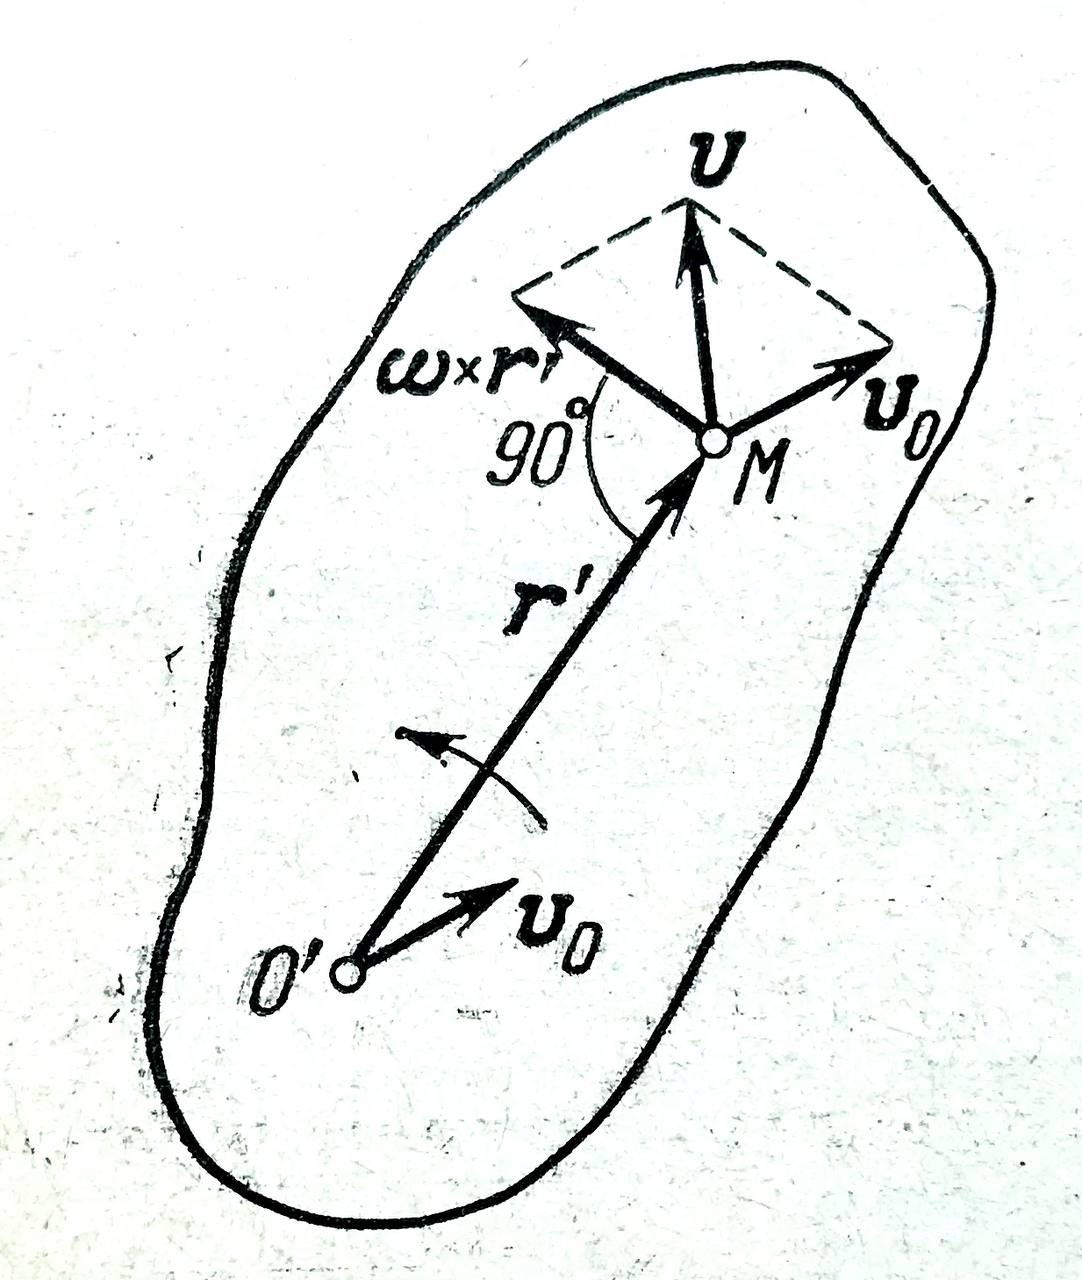
\includegraphics{src/mechanics/pictures/16_1.jpg}}

  \caption{}
  \label{fig:16_1}
\end{figure}

Рассмотрим два частных случая.
\begin{enumerate}
  \item Поступательное движение: $\omega = 0$; формула \ref{eq:figure_velocity}
    даёт
    \begin{equation*}
      \vec{v} = \vec{v}_0,
    \end{equation*}
    то есть скорости всех точек одинаковы и равны скорости полюса.

  \item Вращение вокруг неподвижной оси: $v_0 = 0$; получаем
    \begin{equation*}
      \vec{v} = \crossprod{\vec{\omega}}{\pvec{r}},
    \end{equation*}
    то есть уже известный нам закон распределения скоростей при вращении тела
    вокруг неподвижной оси.
\end{enumerate}

% TODO
(\textcolor{red}{TODO:} в книге на этом месте идут рассуждения об абсолютном,
относительном и переносном движениях. Как мне кажется, оставлять их тут не
надо.)

Дифференцируя по времени уравнение плоского движения $\vec{r} = \vec{r}_0 +
\pvec{r}$, получим
\begin{equation*}
  \vec{v} = \dt[\vec{r}_0] + \dt[\pvec{r}];
\end{equation*}
но первое слагаемое представляет собой скорость полюса и, следовательно,
\begin{equation}
  \label{eq:rotational_velocity}
  \dt[\pvec{r}] = \vec{v} - \vec{v}_0 = \crossprod{\vec{\omega}}{\pvec{r}},
\end{equation}
то есть вращательная скорость вокруг полюса равна производной вектор-радиуса
$\pvec{r}$ по времени.

Формула скорости точки $B$, когда за полюс принята точка $A$, будем обозначать
следующим образом:
\begin{equation}
  \label{eq:figure_velocity_named}
  \vec{v}_B = \vec{v}_A + \vec{v}_{AB}, \quad \vec{v}_{AB} =
    \crossprod{\vec{\omega}}{\pvec{r}_{AB}}.
\end{equation}

\begin{theorem}
  Проекции скоростей концов отрезка на направление отрезка равны между собой.
\end{theorem}

\begin{proof}
  \begin{figure}[H]
    \centering
    \resizebox{\linewidth}{!}
      {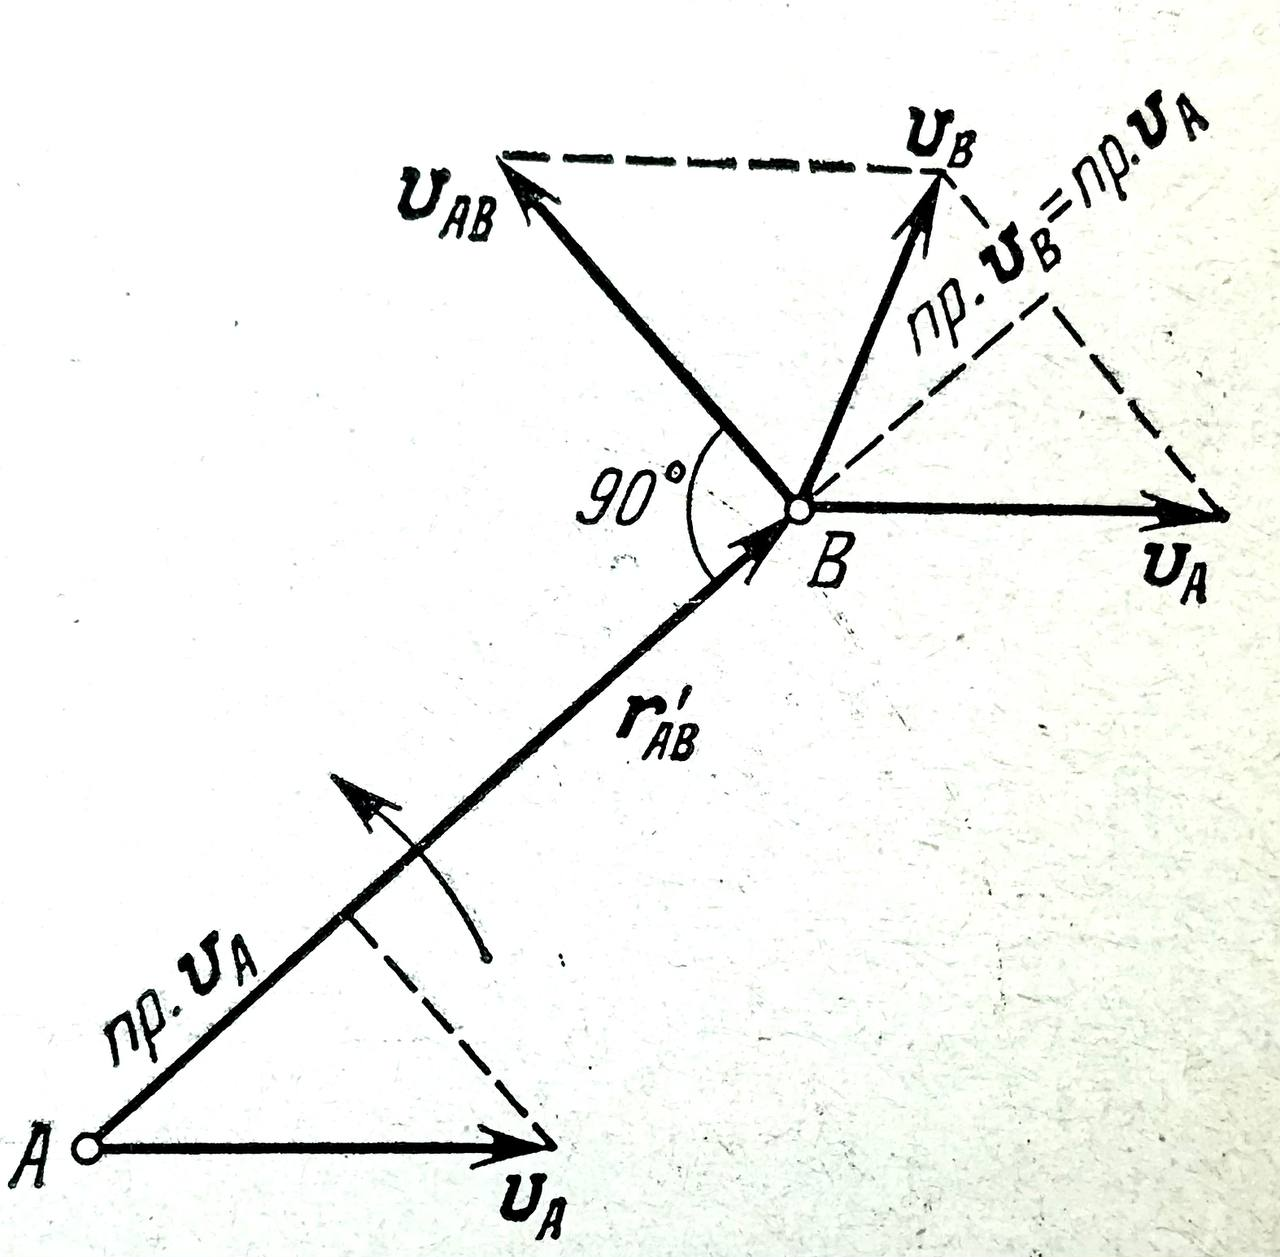
\includegraphics{src/mechanics/pictures/16_2.jpg}}

    \caption{}
    \label{fig:16_2}
  \end{figure}

  По формуле \ref{eq:figure_velocity_named} будем иметь, проектируя обе её части
  на направление отрезка $AB$:
  \begin{equation*}
    \proj_{AB} \vec{v}_B = \proj_{AB} \vec{v}_A + \proj_{AB} \vec{v}_{AB};
  \end{equation*}
  но вектор $\vec{v}_{AB}$ перпендикулярен к направлению отрезка $AB$,
  следовательно, $\proj_{AB} \vec{v}_{AB} = 0$, и окончательно получим
  \begin{equation*}
    \proj_{AB} \vec{v}_B = \proj_{AB} \vec{v}_A.
  \end{equation*}
\end{proof}

\subsection{Список литературы}
\begin{enumerate}
  \item \cite{lourie}
\end{enumerate}

